\section{Linear Classification}
% ============================================================
% SLIDE 1: Giới thiệu
% ============================================================
\begin{frame}[shrink=40]{Linear Classification: Giới thiệu}
    \begin{columns}[T]
        \begin{column}{.5\textwidth}
            \begin{block}{Phát biểu bài toán}
                Cho một tập các quan sát:
                \[
                    \mathcal{D} =  \{(x_1, y_1), \dots, (x_N, y_N)\}
                    \mid x_i \in \textbf{X} \subset \mathbb{R}^p,
                    y_i \in \mathbf{\Pi} = \{\pi_1, \dots, \pi_g\}.
                \]
                Mục tiêu của bài toán phân loại tuyến tính gồm:
                \begin{enumerate}
                    \item \textbf{Seperation:} Tìm một \textbf{biệt thức} phân cách tập dữ liệu tốt nhất.
            
                    \textit{Trong phân loại tuyến tính, biệt thức là một tổ hợp tuyến tính} $\textbf{w}^T \textbf{x}_i$.
                    
                    \item \textbf{Allocation:} Sắp xếp một quan sát $\textbf{x}_0$ vào một trong các nhãn đã định thông qua hàm quyết định $\textbf{f}(.)$.
                \end{enumerate}
            \end{block}
            \begin{block}{Công thức}
                Lớp dự đoán $\hat{\textbf{y}_i}$ của quan sát $\textbf{x}_0$ trong bài toán phân loại tuyến tính được khái quát hóa thành:
                \[ 
                    \hat{y_i} = f(w^Tx_i)
                \]
            \end{block}

        \end{column}

        \begin{column}{.48\textwidth}
            % \vspace*{1cm}
            \begin{exampleblock}{Ví dụ: Phân loại tuyến tính}
                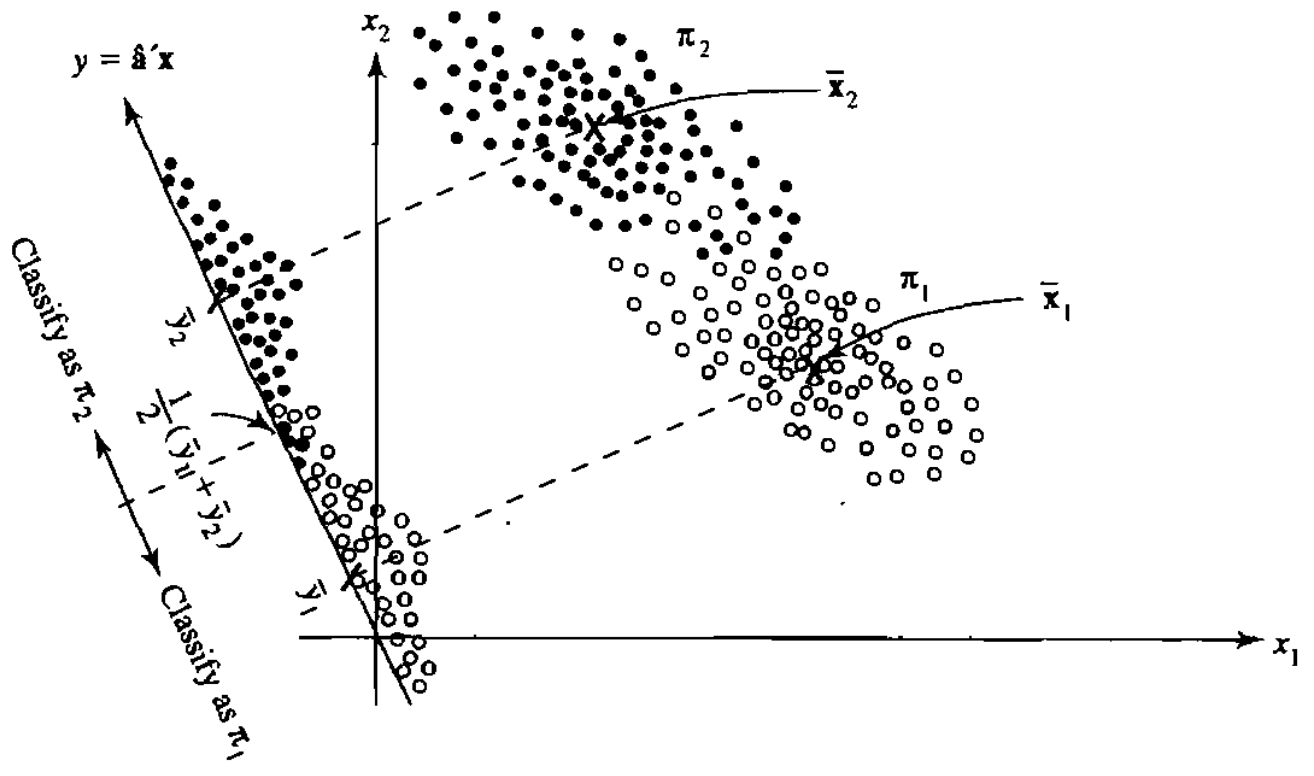
\includegraphics[width=\linewidth]{img/linear}
                
            \end{exampleblock}
        \end{column}
    \end{columns}
\end{frame}

% ============================================================
% SLIDE 2: Naive
% ============================================================
\begin{frame}[shrink=40]{Linear Classification: Biệt thức ngây thơ}
    \begin{columns}[T]
        \begin{column}{.38\textwidth}
            \begin{exampleblock}{Ví dụ: một biệt thức tốt}
                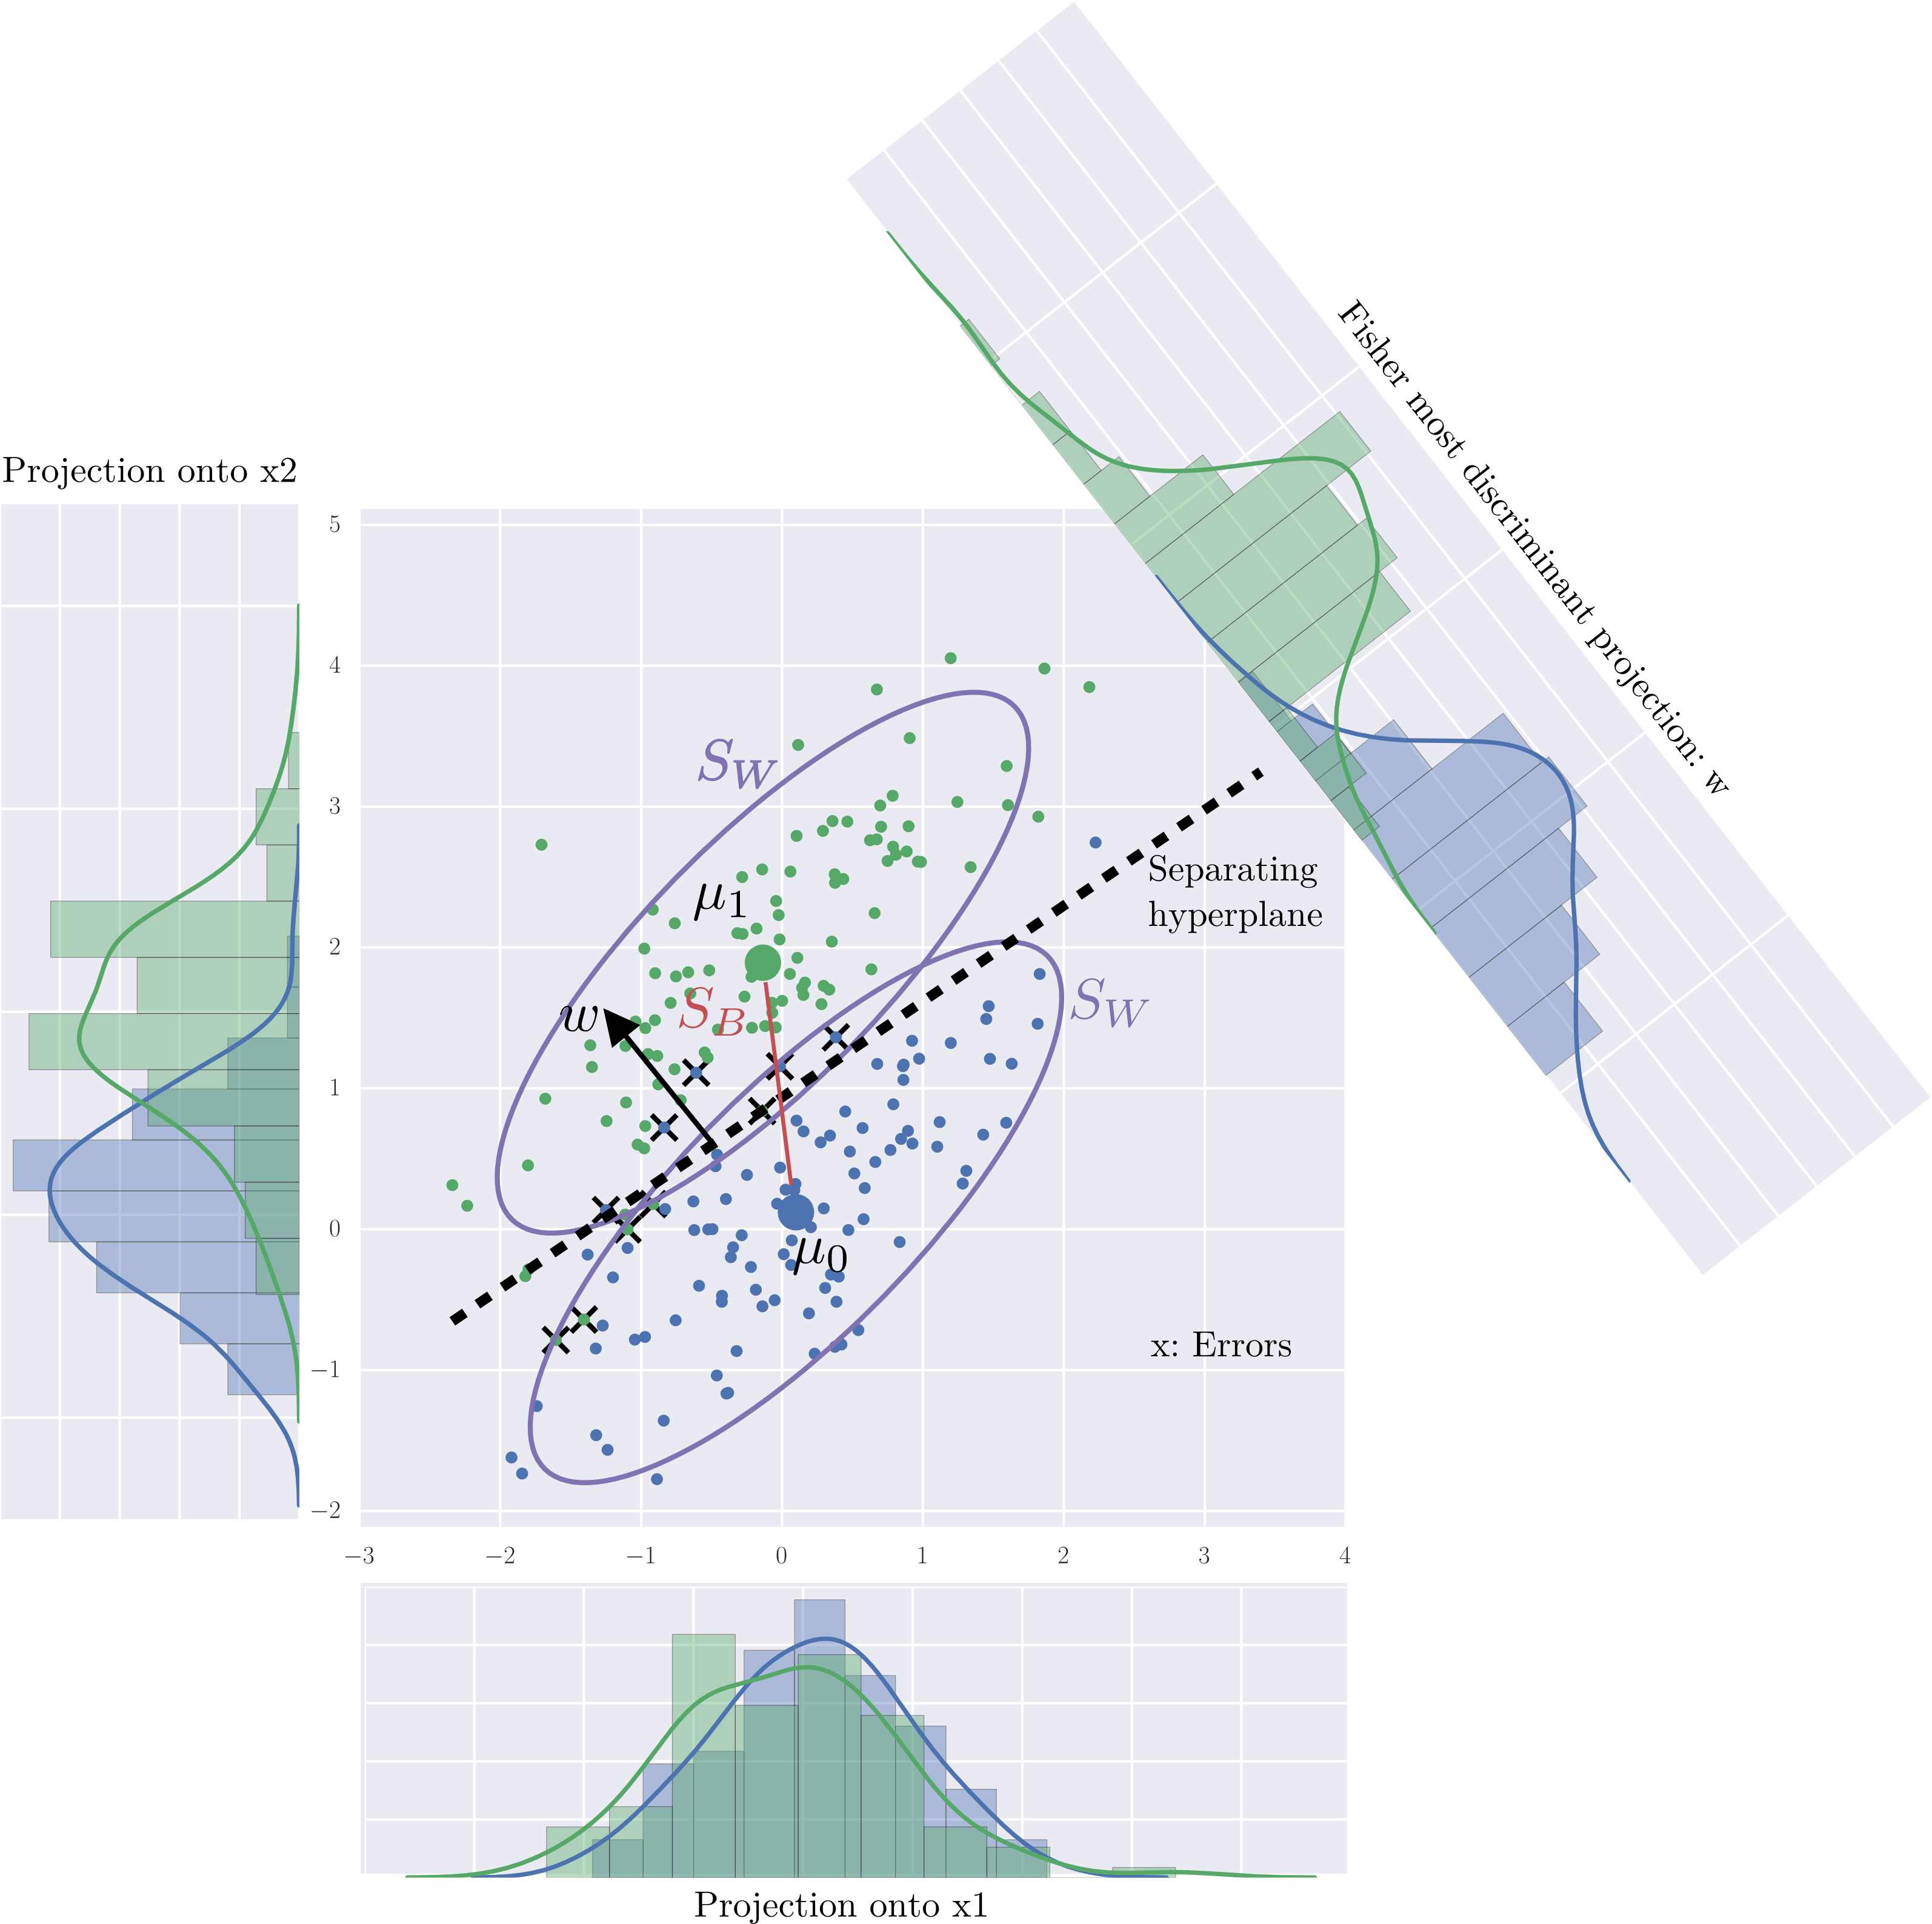
\includegraphics[width=\linewidth]{img/fisher_linear_disc}
            \end{exampleblock}
        \end{column}

        \begin{column}{.60\textwidth}
            \begin{block}{Naive Discriminant}
                Xét trường hợp phân lớp nhị phân $\textbf{g} = 2$
                Biệt thức ngây thơ $\mathbf{w_{Naive}}$ định nghĩa \textbf{seperation} = $|E(x_2) - E(x_1)|$\\
                \vspace*{.5cm}

                Khi ấy, \textbf{seperation} cực đại khi
                    $$ w_{Naive} (= E(x_2) - E(x_1)) = \mu_2 - \mu_1 $$
                
                biến x được chiếu nhận giá trị:
                    $$ x_i = w^Tx_i $$
                \vspace*{4pt}
            \end{block}

            \begin{alertblock}{\textbf{Vấn đề}}
                Biệt thức ngây thơ chỉ quan tâm đến khoảng cách giữa hai trung bình của lớp mà bỏ qua \textbf{hình dạng phân bố của dữ liệu}

                \textbf{Hệ quả:} Dù biệt thức "phân tách tốt" trung bình của từng lớp, song, dữ liệu giữa hai lớp vẫn bị chồng chéo nhau trên không gian chiếu.
            \end{alertblock}
        \end{column}
    \end{columns}
\end{frame}

% ============================================================
% SLIDE 3: Fisher - seperation
% ============================================================
\begin{frame}[shrink=40]{Linear Classification: Biệt thức Fisher}
    \begin{columns}[T]
        \begin{column}{.49\textwidth}
            \begin{block}{Fisher's Discriminant}
                Nhằm giải quyết nhược điểm của \textbf{Biệt thức ngây thơ}, phương pháp của Fisher định nghĩa lại \textbf{seperation}:
                    $$ \textbf{seperation} = \frac{(\text{khoảng cách giữa hai trung bình})}{(\text{độ lệch của mẫu})} = \frac{\lvert \bar{y_1} - \bar{y_2} \rvert}{s_y} $$
                Trong đó:
                \begin{itemize}
                    \item $\textbf{y}_i = w^T x_i w\mid x_i: \text{biến thuộc lớp} \hspace*{4pt} \pi_i$
                    \item $\textbf{s}_y^2 = \frac{\sum_{j = 1}^{n_1}(y_1 - \bar{y}_1)^2 + \sum_{j = 1}^{n_2}(y_2 - \bar{y}_2)^2}{n_1 + n_2 - 2}$
                \end{itemize}
                Ta cần tìm \textbf{w} sao cho \textbf{seperation} là lớn nhất:

                Cho $D^2 = (\textbf{seperation})^2 = \frac{(w^Td)^2}{w^TS_ww}, \hspace*{.25cm}
                \text{với} \hspace*{.25cm} d = \lvert \mu_1 - \mu_2 \rvert:$
                    $$ D^2 \overset{\text{Cauchy-Schwarz mở rộng}}{\leq}
                    \frac{(w^TS_ww)[d^TS_w(x)^{-1}d]}{w^TS_ww}
                    = d^TS_w^{-1}d $$

                    $$ \textbf{"="} \Leftrightarrow \boxed{w \propto S_w^{-1}d} $$
                
                \vspace{4pt}
                    
            \end{block}
        \end{column}

        \begin{column}{.49\textwidth}
            \begin{exampleblock}{Ví dụ: so sánh giữa Naive và Fisher's Discriminant}
                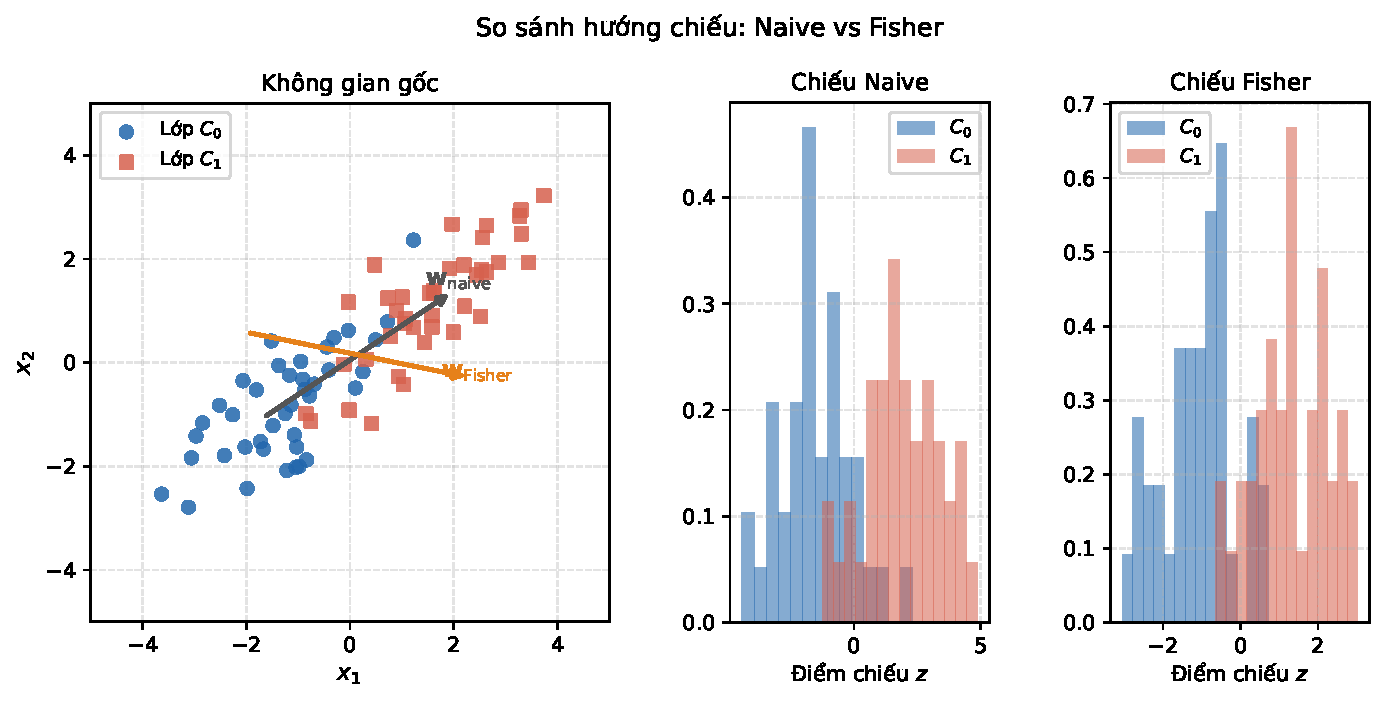
\includegraphics[width=\linewidth]{img/fisher_linear_example}
            \end{exampleblock}
            
            \begin{alertblock}{Nguyên lý}
                \begin{itemize}
                    \item Giả định toàn bộ dữ liệu có chung một "ma trận phương sai trong lớp" ($\textbf{S}_w$)
                    \item \textbf{seperation} đạt cực đại khi $w$ có phương trùng với $S_w^{-1}(\mu_1 - \mu_2)$
                \end{itemize}
            \end{alertblock}
        \end{column}
    \end{columns}
\end{frame}

% ============================================================
% SLIDE 4: Lựa chọn siêu phẳng phân tách
% ============================================================
\begin{frame}[shrink=40]{Linear Classification: Lựa chọn siêu phẳng phân tách tối ưu}
    \begin{columns}[T]
        \begin{column}{.58\textwidth}
            \begin{block}{\textbf{Allocation}: Chọn ngưỡng phân tách}
                Rất khó để tránh "phân lớp sai lầm", nên khi lựa chọn siêu phẳng phân tách, ta dựa trên \textbf{Expected Cost of Misclassification (ECM)} để tính toán những sai lầm ấy:
                \[
                    \boxed{\textbf{ECM} = c(2|1)\,P(2|1)\,p_1 + c(1|2)\,P(1|2)\,p_2}
                \]
                trong đó:
                \begin{itemize}
                    \item $\textbf{c}(i|j)$: chi phí khi nhầm $\pi_j$ thành $\pi_i$
                    \item $\textbf{p}_k$: xác suất tiền nghiệm (prior) của $\pi_k$
                    \item $\textbf{P}(i|j)$: xác suất nhầm $\pi_j$ thành $\pi_i$
                \end{itemize}
                \vspace{.5cm}

                \textbf{Nguyên tắc phân lớp:}\\
                Cho biến ngẫu nhiên $x \in \mathbb{R}^p$:
                \[
                    \pi(x) =
                    \begin{cases}
                        \pi_1 & \text{nếu } (w^*)^Tx - \hat{m} \geq 0   \\
                        \pi_2 & \text{nếu } (w^*)^Tx - \hat{m} < 0
                    \end{cases}
                    , \hspace{.5cm} \hat{m} = (w^*)^T \times \frac{\mu_1 + \mu_2}{2}
                \]


                Nguyên tắc trên ứng với một trường hợp dặc biệt của \textbf{ECM}.
            \end{block}
        \end{column}

        \begin{column}{.38\textwidth}
            \begin{exampleblock}{Ví dụ: siêu phẳng phân tách}
                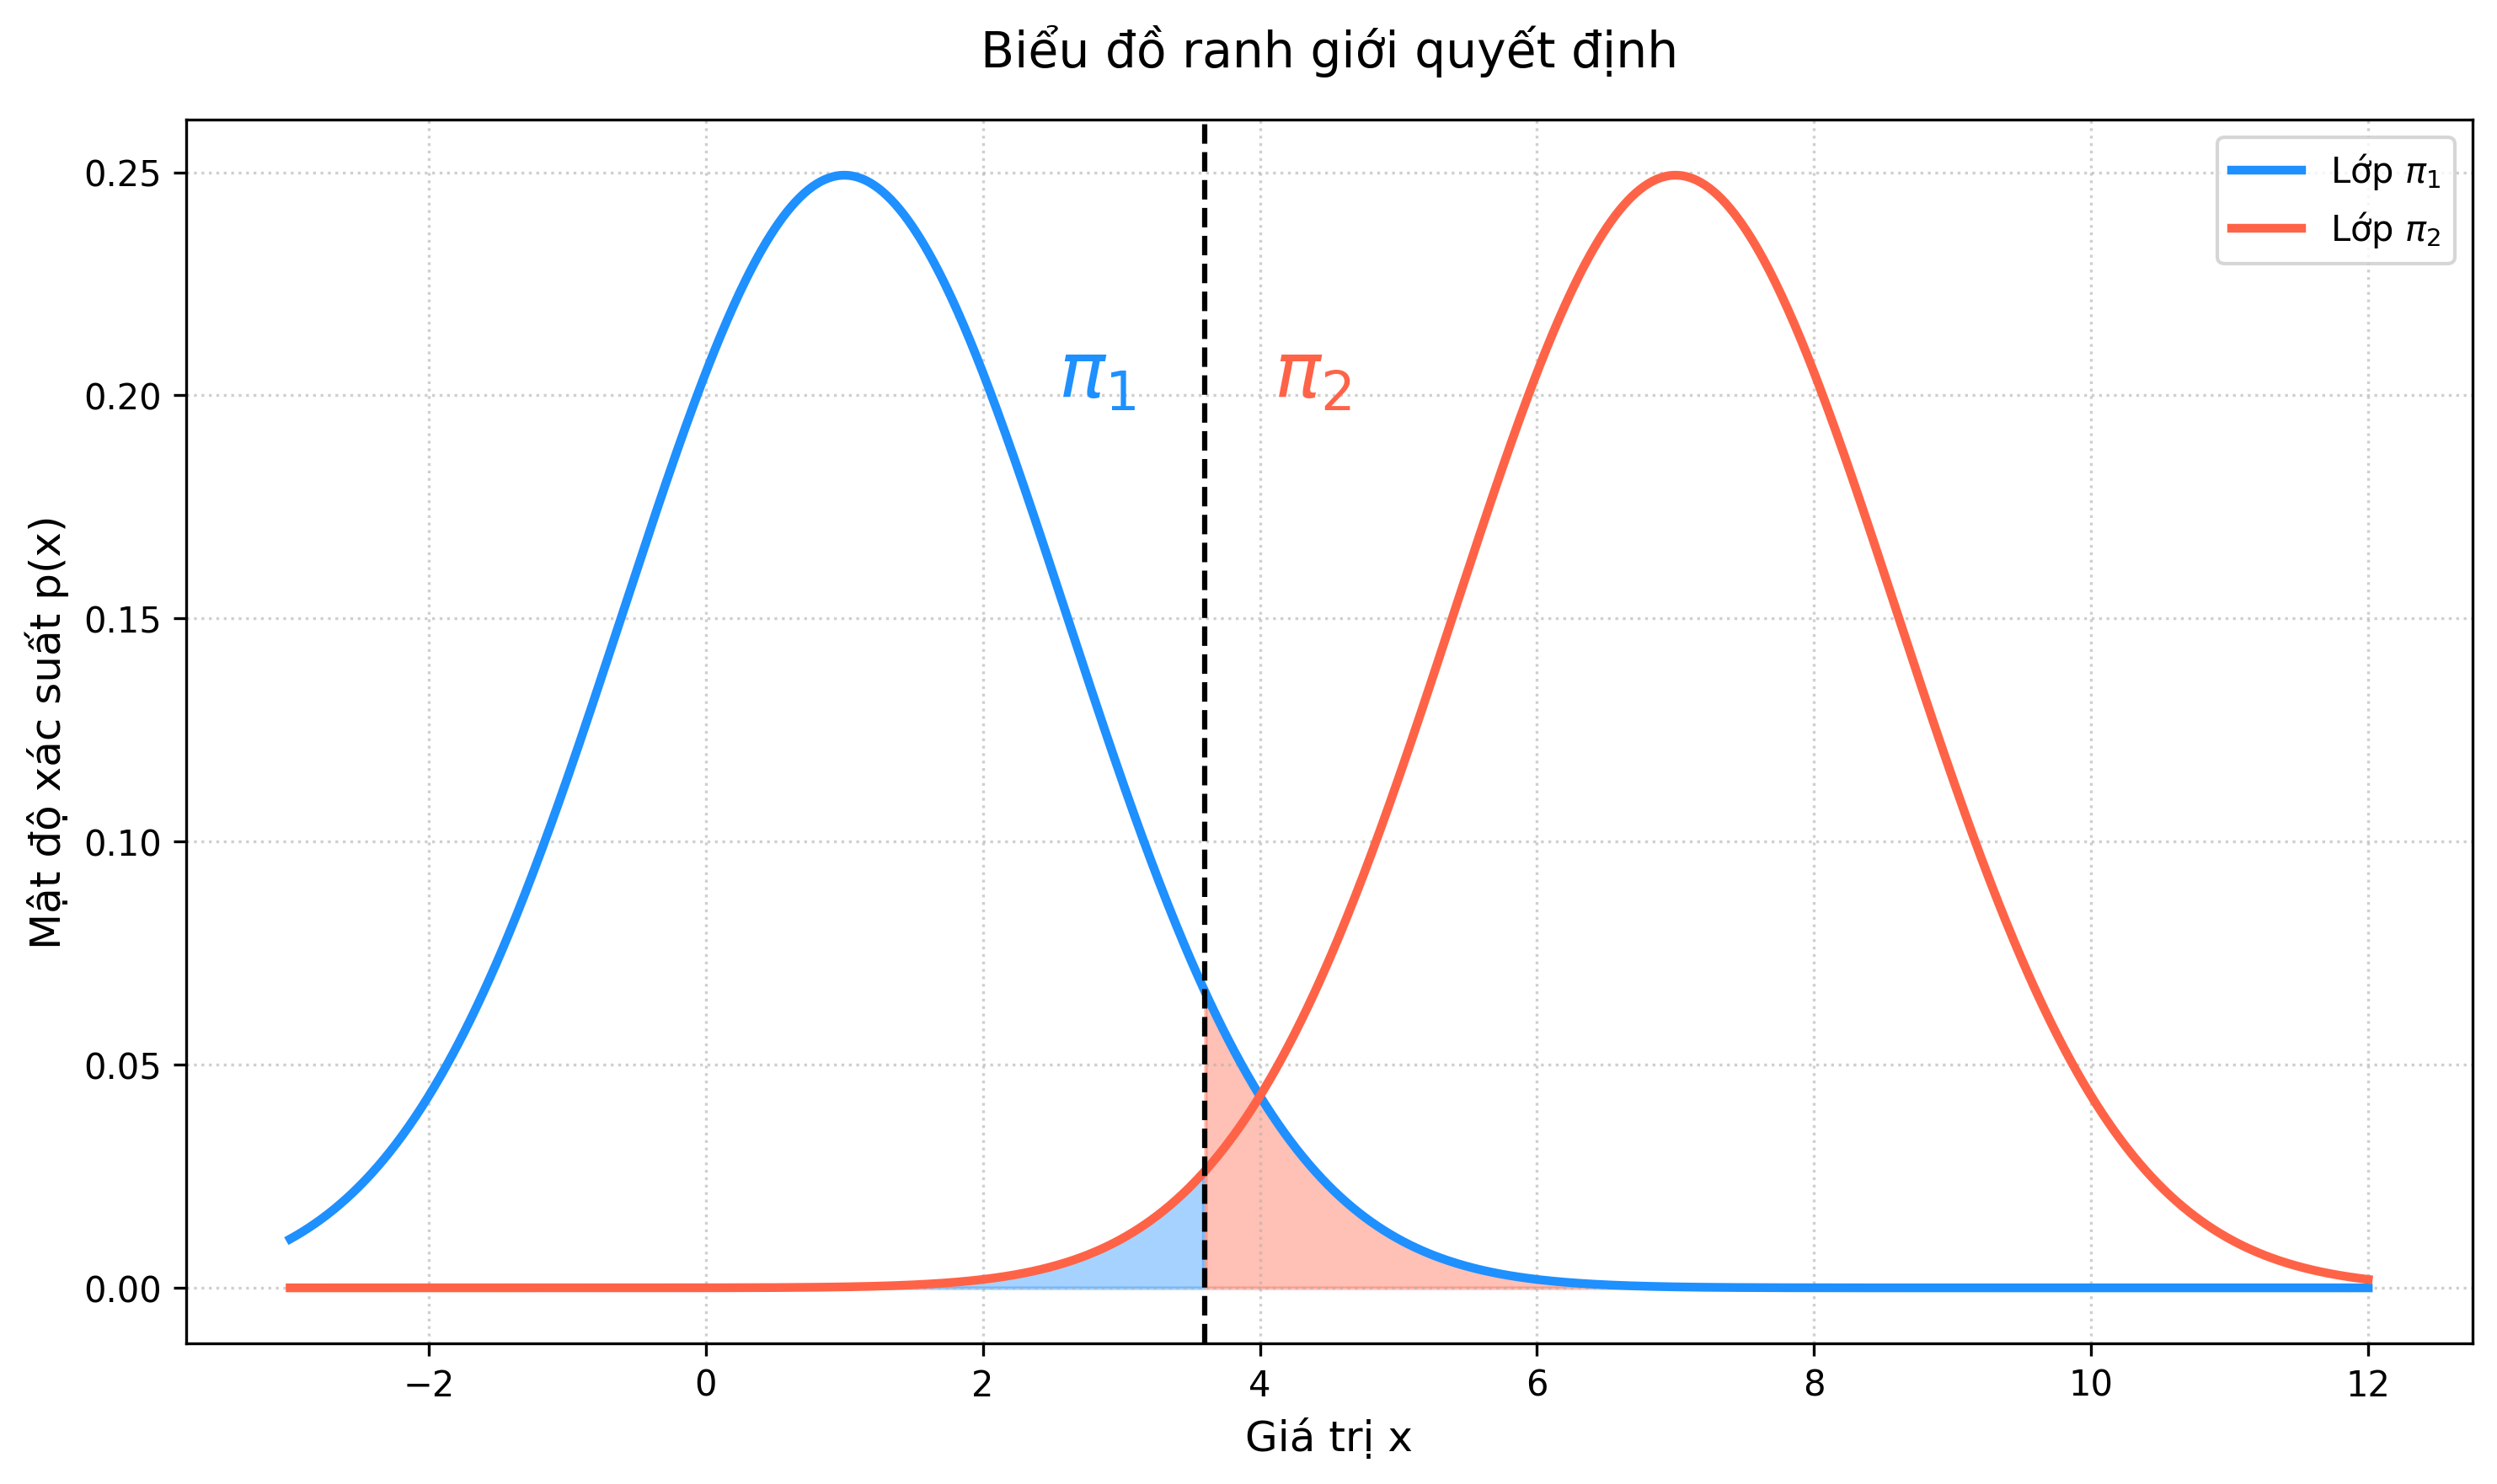
\includegraphics[width=\linewidth]{img/decision_boundary_plot}
            \end{exampleblock}

            \begin{alertblock}{Nguyên lý}
                \begin{itemize}
                    \item Tối thiểu hóa \textbf{"chi phí phân loại sai" (ECM)}.
                    \item \textbf{Hàm biệt thức tuyến tính Fisher} thông thường tương ứng với tối ưu \textbf{ECM} có \textbf{chi phí sai lầm} và \textbf{xác suất tiền nghiệm} bằng nhau.
                \end{itemize}
            \end{alertblock}
        \end{column}
    \end{columns}
\end{frame}

% ============================================================
% SLIDE 5: Chứng minh ECM
% ============================================================
\begin{frame}[shrink=40]{Linear Classification: Lựa chọn siêu phẳng phân tách tối ưu}
    \begin{columns}[T]
        \begin{column}{.58\textwidth}
            \begin{block}{\textbf{Chứng minh}: ECM nhỏ nhất khi $p_1 = p_2$, $c(2|1) = c(1|2)$}
                \vspace{.5cm}
                \textbf{Gọi} $R_k$ \textbf{là không gian dự đoán lớp} $\pi_k$. Khi $p_1 = p_2$ và $c(2|1) = c(1|2)$:
                \begin{align*}
                    ECM &\propto P(2|1) + P(1|2) \\
                        &= \int_{R_2} f_1(x)\,dx + \int_{R_1} f_2(x)\,dx \\
                        &= \int_{\Omega} f_1(x)\,dx - \int_{R_1} f_1(x)\,dx
                           + \int_{R_1} f_2(x)\,dx \\
                        &= 1 + \int_{R_1} \bigl[f_2(x) - f_1(x)\bigr]\,dx
                \end{align*}

                \vspace{.5cm}
                ECM tối thiểu khi: \hspace{59pt}$R_1 = \bigl\{x : f_1(x) \geq f_2(x)\bigr\}$

                Chứng minh tương tự, ta được: $R_2 = \bigl\{x : f_1(x) \leq f_2(x)\bigr\}$
                
                \vspace{.5cm}
                Vậy, biên quyết định nằm ở $ x_0:f_1(x_0) = f_2(x_0) \hspace{.5cm} \Leftrightarrow \hspace{.5cm} x_0 = \frac{\mu_1 + \mu_2}{2}$
                \vspace{.5cm}
            \end{block}
        \end{column}

        \begin{column}{.38\textwidth}
            \begin{exampleblock}{Ví dụ: trường hợp tối ưu}
                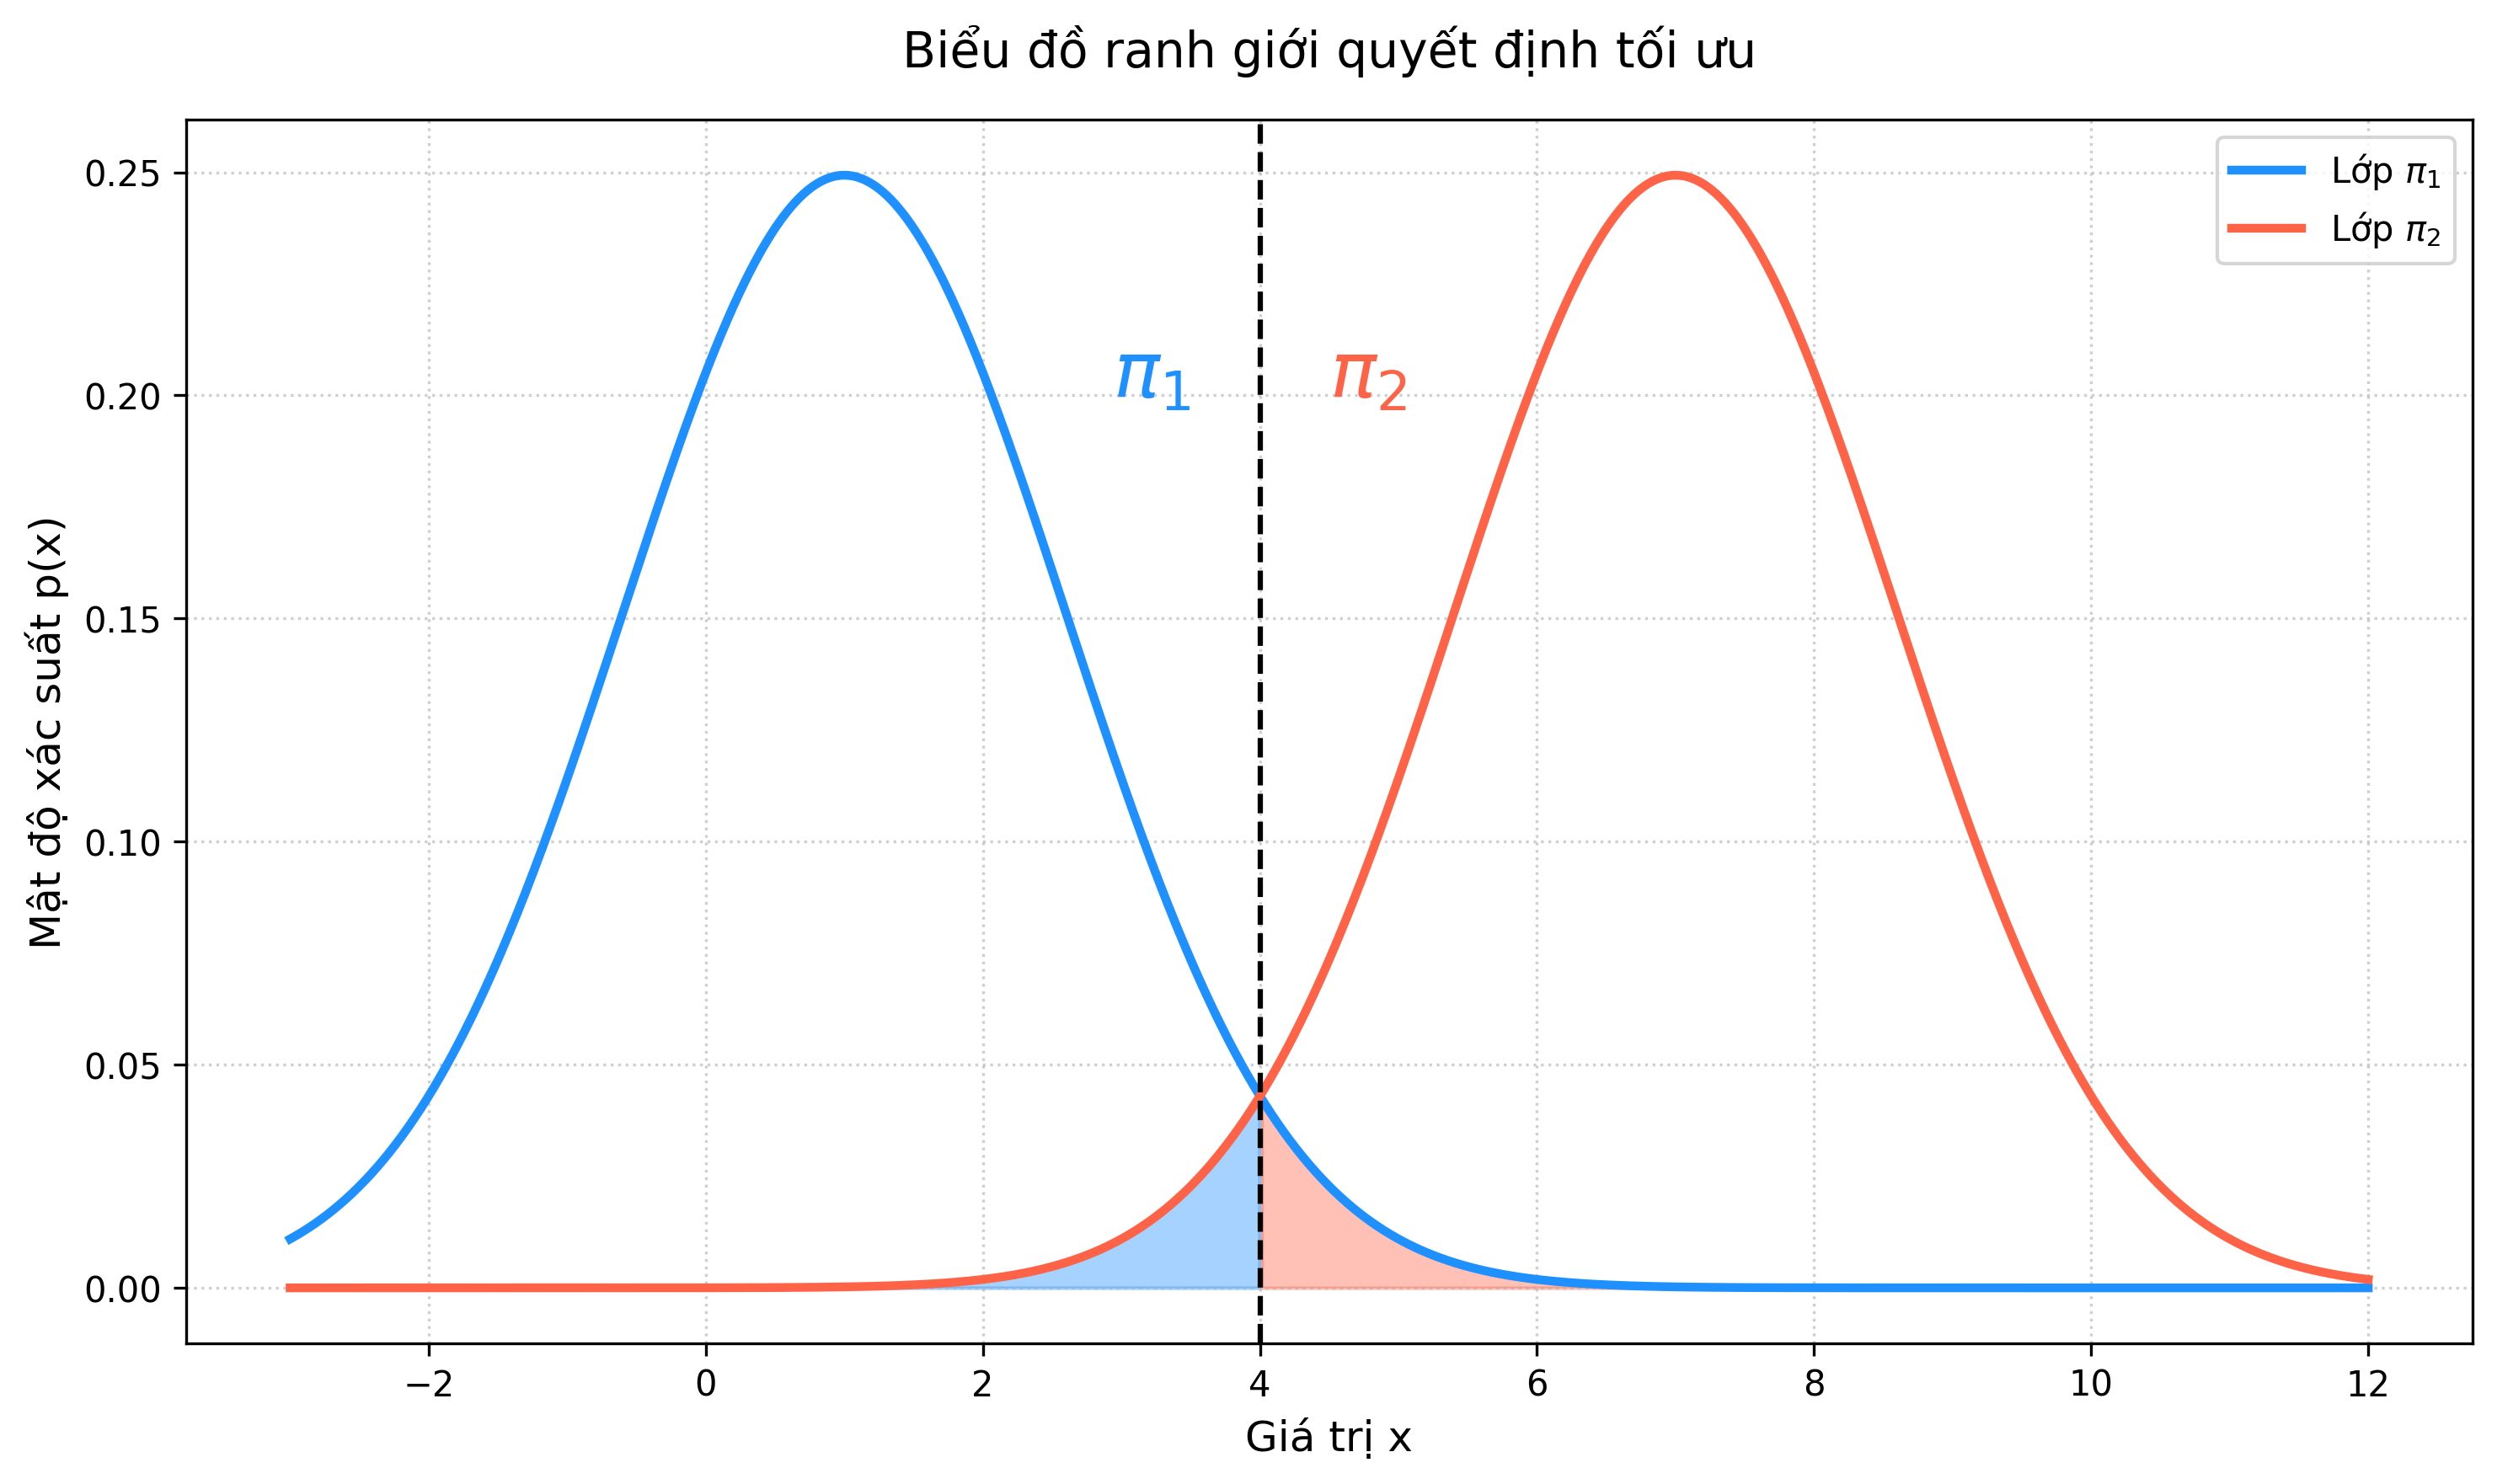
\includegraphics[width=\linewidth]{img/optimal_decision_boundary_plot}
            \end{exampleblock}

            \begin{alertblock}{Nguyên lý}
                \begin{itemize}
                    \item Tối thiểu hóa \textbf{"chi phí phân loại sai" (ECM)}.
                    \item \textbf{Hàm biệt thức tuyến tính Fisher} thông thường tương ứng với tối ưu \textbf{ECM} có \textbf{chi phí sai lầm} và \textbf{xác suất tiền nghiệm} bằng nhau.
                \end{itemize}
            \end{alertblock}
        \end{column}
    \end{columns}
\end{frame}

% ============================================================
% SLIDE 6: LDA introduction 
% ============================================================

\begin{frame}[shrink=40]{Linear Classification: Phân tích biệt thức tuyến tính(LDA)}
    \begin{columns}[T]
        \begin{column}{0.7\textwidth}
            \begin{block}{Linear Discriminant Analysis}
                \textbf{Giả định:} Mỗi lớp $\pi_k$ có phân phối chuẩn đa biến:
                $$ x \mid y = \pi_k \sim \mathcal{N}(\mu_k, \Sigma) $$
                trong đó \textbf{tất cả các lớp chia sẻ chung ma trận hiệp phương sai} $\Sigma$.

                \vspace{0.3cm}
                \textbf{Hàm biệt thức tuyến tính} cho lớp $\pi_k$:
                $$ \delta_k(x) = x^T \Sigma^{-1} \mu_k - \frac{1}{2}\mu_k^T \Sigma^{-1}\mu_k + \ln p_k $$
                trong đó $p_k = P(\pi_k)$ là xác suất tiền nghiệm.

                \vspace{0.3cm}
                \textbf{Quy tắc phân lớp Bayes:}
                $$ \hat{y} = \arg\max_{k} \; \delta_k(x) $$
                
                \vspace{0.2cm}
                Với $g = 2$, biên quyết định $\delta_1(x) = \delta_2(x)$:
                $$ x^T \Sigma^{-1}(\mu_1 - \mu_2) = \frac{1}{2}(\mu_1 + \mu_2)^T \Sigma^{-1}(\mu_1 - \mu_2) - \ln\frac{p_1}{p_2} $$
            \end{block}

        \end{column}

        \begin{column}{0.28\textwidth}
            \begin{exampleblock}{Ví dụ: LDA trên 2 lớp Gaussian}
                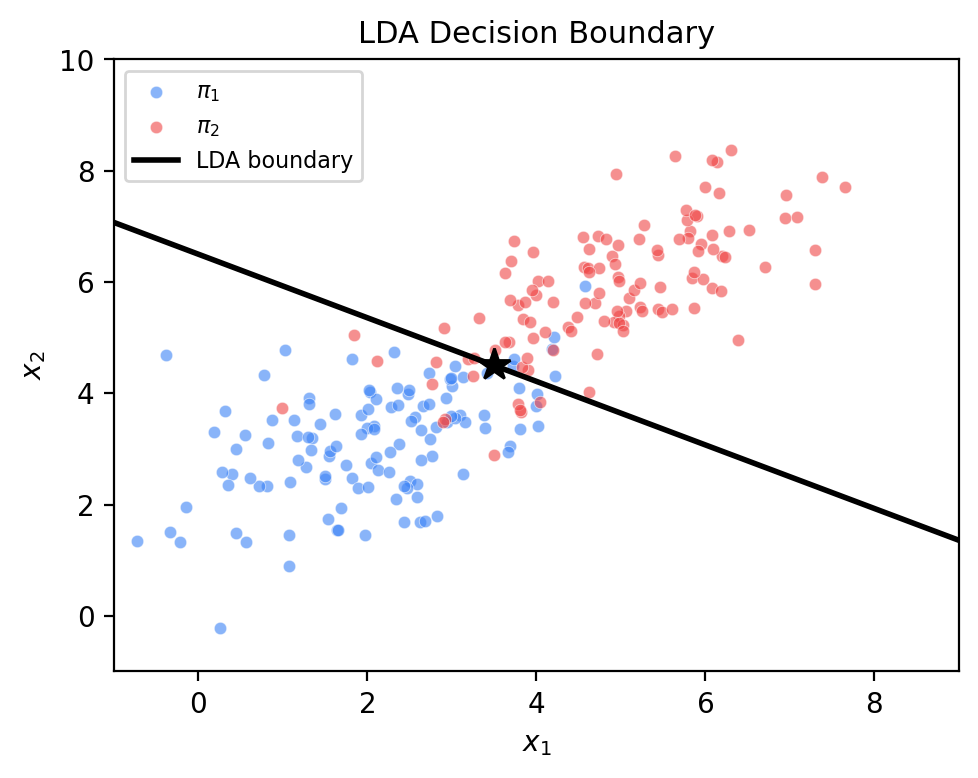
\includegraphics[width=\linewidth]{img/lda_example}
            \end{exampleblock}

            \begin{alertblock}{Nguyên lý}
                \begin{itemize}
                    \item Maximum likelihood Discriminant: LDA chính là phân lớp Bayes tối ưu dưới giả định Gaussian chung $\Sigma$.
                    \item $\delta_k(x)$ tuyến tính theo $x$ $\Rightarrow$ biên quyết định là \textbf{siêu phẳng}.
                \end{itemize}
            \end{alertblock}
        \end{column}
    \end{columns}
\end{frame}


% ============================================================
% SLIDE 7: ECM of LDA, comparison with Fisher
% ============================================================

\begin{frame}[shrink=40]{Linear Classification: Liên hệ giữa LDA và Fisher}
    \begin{columns}[T]
        \begin{column}{0.58\textwidth}
            \begin{block}{Chứng minh: LDA $\equiv$ Fisher khi $\Sigma$ chung}
                \textbf{Từ Fisher:} $w^* \propto S_w^{-1}(\mu_1 - \mu_2)$

                \vspace{0.3cm}
                \textbf{Từ LDA} (Bayes với Gaussian chung $\Sigma$):
                \begin{align*}
                    \delta_1(x) &= \delta_2(x) \\
                    \Leftrightarrow \quad x^T\Sigma^{-1}(\mu_1 - \mu_2) &= \text{const}
                \end{align*}
                Hướng pháp tuyến của biên quyết định:
                $$ w_{LDA} \propto \Sigma^{-1}(\mu_1 - \mu_2) $$

                \vspace{0.3cm}
                Vì $S_w$ là ước lượng không chệch của $\Sigma$:
                $$ S_w = \frac{1}{n_1 + n_2 - 2}\sum_{k=1}^{2}\sum_{x_i \in \pi_k}(x_i - \bar{x}_k)(x_i - \bar{x}_k)^T $$

                $$ \Rightarrow \boxed{w_{Fisher} \propto S_w^{-1}d \;\approx\; \Sigma^{-1}(\mu_1 - \mu_2) \propto w_{LDA}} $$
            \end{block}
        \end{column}

        \begin{column}{0.4\textwidth}
            \begin{exampleblock}{Ví dụ: Fisher $\equiv$ LDA}
                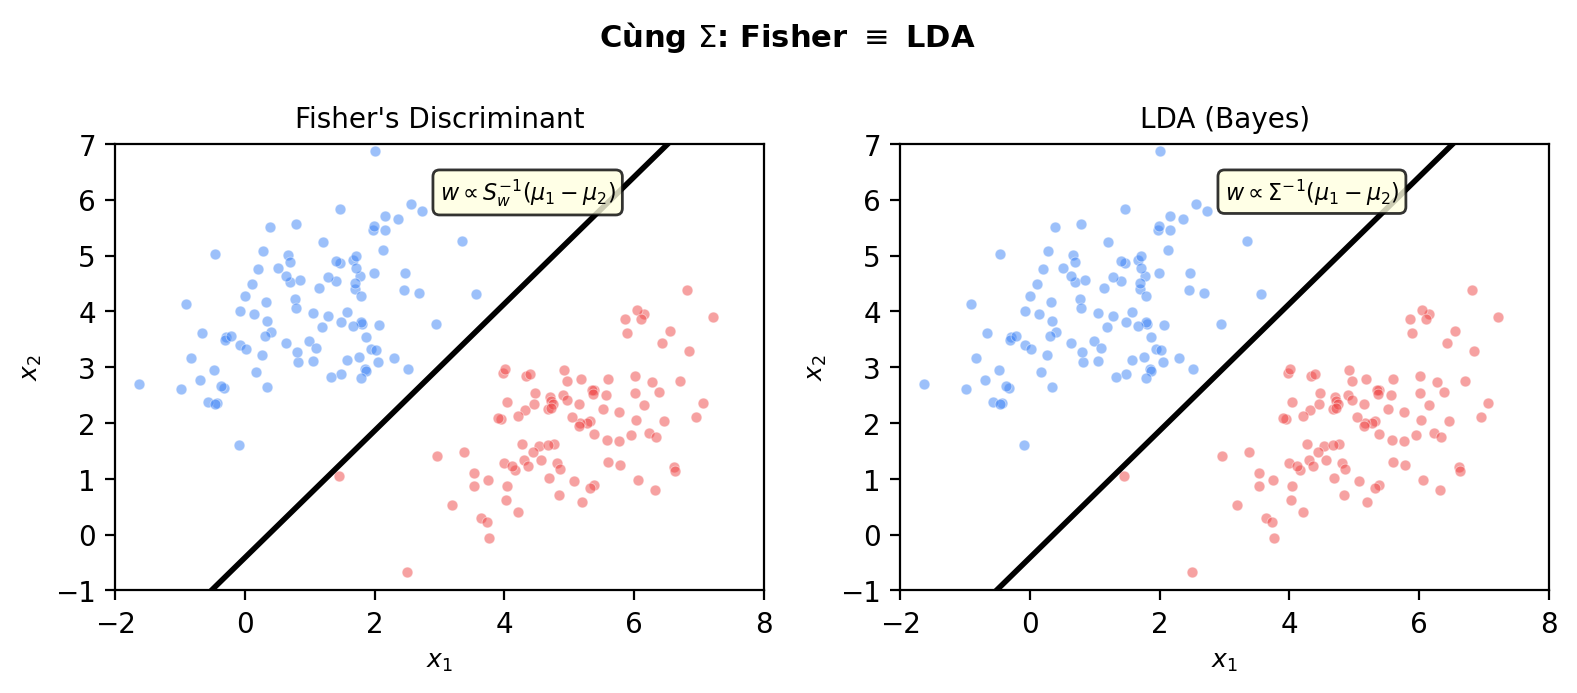
\includegraphics[width=\linewidth]{img/lda_fisher_equiv}
            \end{exampleblock}

            \begin{alertblock}{Nguyên lý}
                \begin{itemize}
                    \item Khi các lớp có chung $\Sigma$, Fisher's Discriminant và LDA cho \textbf{cùng hướng phân tách} $w$.
                    \item Fisher: tiếp cận \textbf{hình học} (cực đại separation). LDA: tiếp cận \textbf{xác suất} (Bayes).
                \end{itemize}
            \end{alertblock}
        \end{column}
    \end{columns}
\end{frame}

% ============================================================
% SLIDE 8: LDA with view of ECM, comparison with Fisher
% ============================================================

\begin{frame}[shrink=40]{Linear Classification: LDA dưới góc nhìn ECM}
    \begin{columns}[T]
        \begin{column}{0.58\textwidth}
            \begin{block}{LDA tổng quát: prior và cost không bằng nhau}
                Khi $p_1 \neq p_2$ hoặc $c(2|1) \neq c(1|2)$, quy tắc phân lớp trở thành:
                $$ \pi(x) = \pi_1 \;\; \text{nếu} \;\; \frac{f_1(x)}{f_2(x)} \geq \frac{c(1|2)\,p_2}{c(2|1)\,p_1} $$

                \vspace{0.3cm}
                Lấy $\log$ hai vế (\textbf{log-odds ratio}):
                $$ \ln\frac{f_1(x)}{f_2(x)} \geq \ln\frac{c(1|2)\,p_2}{c(2|1)\,p_1} $$

                \vspace{0.3cm}
                Dưới giả định Gaussian chung $\Sigma$:
                \begin{align*}
                    &x^T\Sigma^{-1}(\mu_1 - \mu_2) - \frac{1}{2}(\mu_1^T\Sigma^{-1}\mu_1 - \mu_2^T\Sigma^{-1}\mu_2) \\
                    &\qquad \geq \ln\frac{c(1|2)\,p_2}{c(2|1)\,p_1}
                \end{align*}

                \vspace{0.2cm}
                Biên quyết định \textbf{dịch chuyển} tuỳ theo tỷ lệ cost/prior.
            \end{block}
        \end{column}

        \begin{column}{0.4\textwidth}
            \begin{exampleblock}{Ví dụ: Dịch chuyển biên quyết định}
                Khi $p_1 > p_2$: biên dịch về phía $\pi_2$ (mở rộng vùng $\pi_1$).\\[0.3cm]
                Khi $c(2|1) > c(1|2)$: ``nhầm $\pi_1$ thành $\pi_2$'' đắt hơn $\Rightarrow$ biên cũng dịch về phía $\pi_2$.
            \end{exampleblock}

            \begin{alertblock}{Nguyên lý}
                \begin{itemize}
                    \item Fisher thông thường $\equiv$ LDA với $p_1 = p_2$, $c(2|1) = c(1|2)$.
                    \item LDA tổng quát hơn: cho phép điều chỉnh biên quyết định theo \textbf{chi phí sai lầm} thực tế.
                \end{itemize}
            \end{alertblock}
        \end{column}
    \end{columns}
\end{frame}

% ============================================================
% SLIDE 9: Nhóm các mô hình Linear Regression
% ============================================================

\begin{frame}[shrink=40]{Linear Classification: Định nghĩa bài toán}
    \begin{columns}[T]
        \begin{column}{0.7\textwidth}
            \begin{block}{Phân lớp bằng Linear Regression}
                \textbf{Ý tưởng:} Mã hoá nhãn thành \textbf{indicator matrix} $\mathbf{Y} \in \{0,1\}^{N \times g}$:
                $$ Y_{ik} = \begin{cases} 1 & \text{nếu } y_i = \pi_k \\ 0 & \text{ngược lại} \end{cases} $$

                \vspace{0.2cm}
                Giải bài toán hồi quy OLS:
                $$ \hat{B} = (X^TX)^{-1}X^TY $$

                Phân lớp: $\hat{y}(x) = \arg\max_k \; \hat{f}_k(x) = \arg\max_k \; x^T\hat{\beta}_k$

                \vspace{0.3cm}
                \textbf{Hạn chế -- Masking:}
                \begin{itemize}
                    \item Khi $g \geq 3$, hồi quy tuyến tính có thể bị \textbf{che khuất (masking)}: một lớp bị "nuốt" bởi vùng quyết định của các lớp khác.
                    \item Giá trị $\hat{f}_k(x)$ \textbf{không bị ràng buộc} trong $[0,1]$ $\Rightarrow$ khó diễn giải như xác suất.
                \end{itemize}
            \end{block}
        \end{column}

        \begin{column}{0.28\textwidth}
            \begin{exampleblock}{Ví dụ: Masking trong 3 lớp}
                Với 3 lớp: hồi quy tuyến tính có thể tạo vùng quyết định sai lệch -- lớp ở giữa bị che khuất hoàn toàn bởi hai lớp ngoài.
            \end{exampleblock}

            \begin{alertblock}{Nguyên lý}
                \begin{itemize}
                    \item OLS cho phân lớp: đơn giản nhưng \textbf{không tối ưu}.
                    \item Cần các mô hình chuyên biệt: Logistic Regression, SVM.
                \end{itemize}
            \end{alertblock}
        \end{column}
    \end{columns}
\end{frame}

% ============================================================
% SLIDE 10: Các hàm mất mát (Loss Function) trong Linear Regression
% ============================================================

\begin{frame}[shrink=40]{Linear Classification: Các hàm mất mát}
    \begin{columns}[T]
        \begin{column}{0.58\textwidth}
            \begin{block}{Loss Functions cho phân lớp}
                Cho $m = y \cdot f(x)$ (\textbf{functional margin}), các hàm loss phổ biến:

                \vspace{0.3cm}
                \textbf{1. 0-1 Loss} (lý tưởng, không khả vi):
                $$ L_{0-1}(m) = \mathbb{1}[m < 0] $$

                \textbf{2. Squared Loss} (dùng trong OLS):
                $$ L_{sq}(m) = (1 - m)^2 $$

                \textbf{3. Hinge Loss} (dùng trong SVM):
                $$ L_{hinge}(m) = \max(0,\; 1 - m) = [1 - m]_+ $$

                \textbf{4. Logistic Loss} (dùng trong Logistic Regression):
                $$ L_{log}(m) = \log_2(1 + e^{-m}) $$

                \vspace{0.2cm}
                Tất cả đều là \textbf{upper bound} của 0-1 loss và \textbf{convex} (trừ 0-1 loss).
            \end{block}
        \end{column}

        \begin{column}{0.4\textwidth}
            \begin{exampleblock}{Ví dụ: So sánh các hàm Loss}
                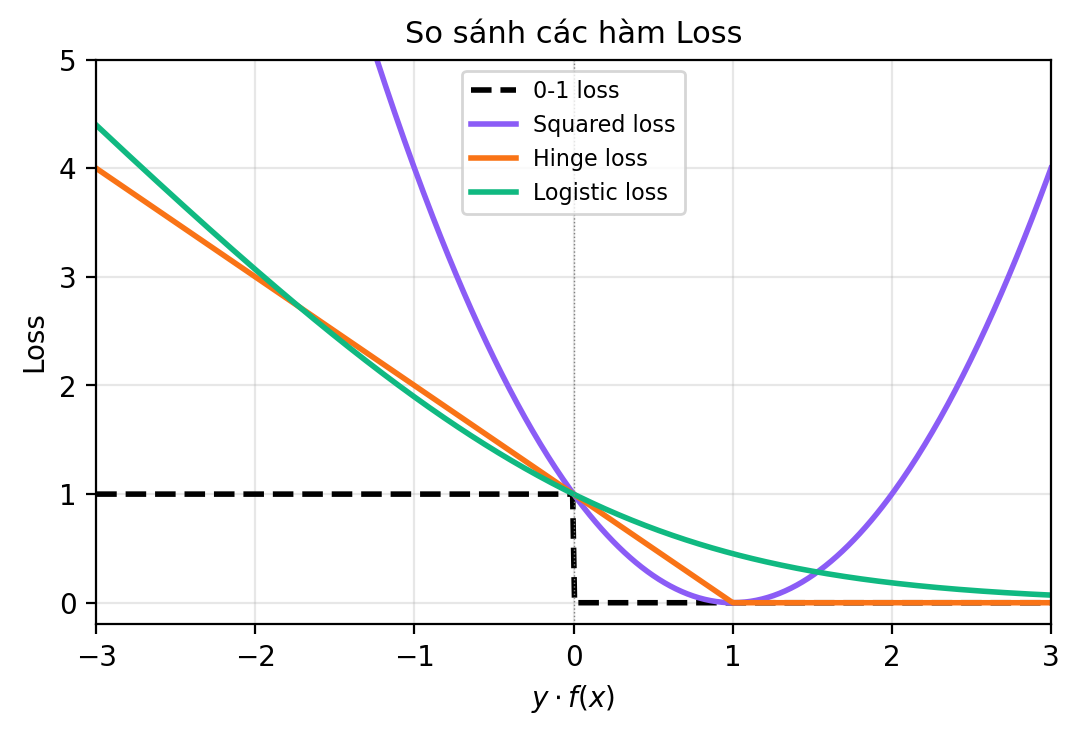
\includegraphics[width=\linewidth]{img/loss_functions}
            \end{exampleblock}

            \begin{alertblock}{Nguyên lý}
                \begin{itemize}
                    \item Chọn loss function $\Leftrightarrow$ chọn mô hình phân lớp.
                    \item Hinge loss: khuyến khích \textbf{margin lớn} (SVM). Logistic loss: cho \textbf{ước lượng xác suất}.
                \end{itemize}
            \end{alertblock}
        \end{column}
    \end{columns}
\end{frame}

% ============================================================
% SLIDE 11: Những hàm điều phối (Regularization Function) trong Linear Regression
% ============================================================

\begin{frame}[shrink=40]{Linear Classification: Điều chuẩn (Regularization)}
    \begin{columns}[T]
        \begin{column}{0.58\textwidth}
            \begin{block}{Regularization Functions}
                Thêm hạng tử phạt vào hàm mục tiêu để \textbf{tránh overfitting}:
                $$ \hat{w} = \arg\min_w \sum_{i=1}^{N} L(y_i, f(x_i)) + \lambda \cdot \Omega(w) $$

                \vspace{0.2cm}
                \textbf{1. L2 -- Ridge} ($\Omega = \|w\|_2^2$):
                $$ \hat{w}_{Ridge} = \arg\min_w \sum L_i + \lambda \sum_{j} w_j^2 $$
                Thu nhỏ hệ số đều, \textbf{không loại bỏ} biến.

                \vspace{0.2cm}
                \textbf{2. L1 -- Lasso} ($\Omega = \|w\|_1$):
                $$ \hat{w}_{Lasso} = \arg\min_w \sum L_i + \lambda \sum_{j} |w_j| $$
                Đẩy một số hệ số \textbf{về đúng 0} $\Rightarrow$ \textbf{chọn biến (sparsity)}.

                \vspace{0.2cm}
                \textbf{3. Elastic Net} ($\Omega = \alpha\|w\|_1 + (1-\alpha)\|w\|_2^2$):
                Kết hợp cả L1 và L2.
            \end{block}
        \end{column}

        \begin{column}{0.4\textwidth}
            \begin{exampleblock}{Ví dụ: L1 vs L2 regularization}
                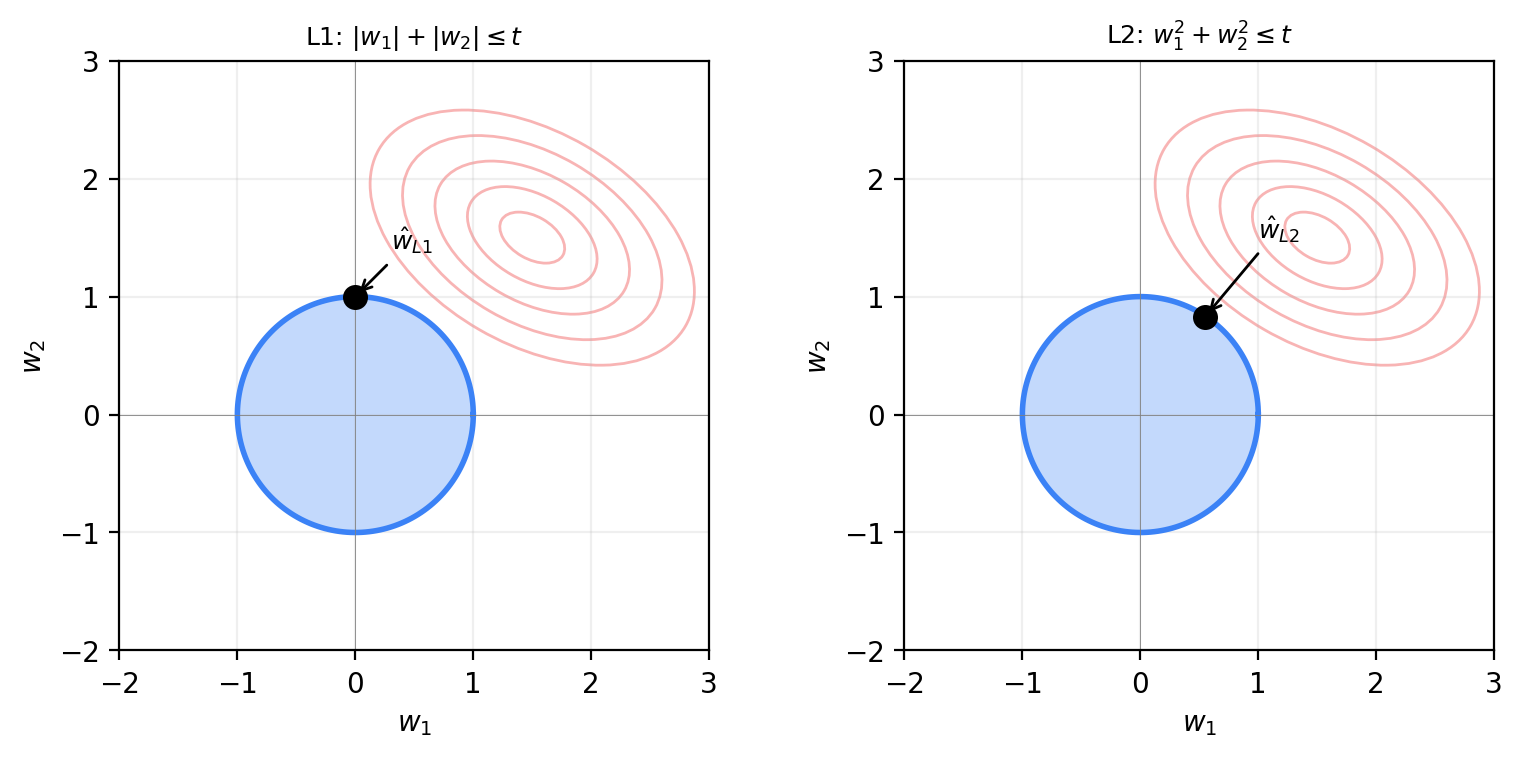
\includegraphics[width=\linewidth]{img/l1_vs_l2}
            \end{exampleblock}

            \begin{alertblock}{Nguyên lý}
                \begin{itemize}
                    \item L1: vùng ràng buộc hình \textbf{thoi} $\Rightarrow$ nghiệm hay rơi vào đỉnh (sparse).
                    \item L2: vùng ràng buộc hình \textbf{tròn} $\Rightarrow$ nghiệm co đều.
                \end{itemize}
            \end{alertblock}
        \end{column}
    \end{columns}
\end{frame}

% ============================================================
% SLIDE 12: Những hàm điều phối (Regularization Function) trong Linear Regression
% ============================================================

\begin{frame}[shrink=40]{Linear Classification: Logistic Regression}
    \begin{columns}[T]
        \begin{column}{0.58\textwidth}
            \begin{block}{Mô hình Logistic Regression}
                Mô hình hoá \textbf{xác suất hậu nghiệm} trực tiếp:
                $$ P(y = 1 \mid x) = \sigma(w^Tx + b) = \frac{1}{1 + e^{-(w^Tx + b)}} $$

                \vspace{0.2cm}
                \textbf{Log-odds} (logit) là tuyến tính theo $x$:
                $$ \ln\frac{P(y=1|x)}{P(y=0|x)} = w^Tx + b $$

                \vspace{0.2cm}
                \textbf{Ước lượng tham số -- MLE:}
                \begin{align*}
                    \ell(w) &= \sum_{i=1}^{N} \bigl[y_i \ln \hat{p}_i + (1-y_i)\ln(1-\hat{p}_i)\bigr] \\
                    \hat{w} &= \arg\max_w \; \ell(w)
                \end{align*}
                Giải bằng \textbf{Gradient Ascent} hoặc \textbf{Newton-Raphson} (IRLS).
            \end{block}
        \end{column}

        \begin{column}{0.4\textwidth}
            \begin{exampleblock}{Ví dụ: Hàm sigmoid $\sigma(z)$}
                \begin{center}
                    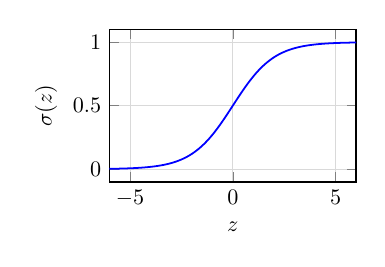
\begin{tikzpicture}[scale=0.8]
                        \begin{axis}[
                            width=5.5cm, height=4cm,
                            xlabel={$z$}, ylabel={$\sigma(z)$},
                            xmin=-6, xmax=6, ymin=-0.1, ymax=1.1,
                            grid=major, grid style={gray!30},
                            thick
                        ]
                        \addplot[blue, domain=-6:6, samples=100] {1/(1+exp(-x))};
                        \addplot[dashed, gray] coordinates {(0,0.5) (0,0.5)};
                        \end{axis}
                    \end{tikzpicture}
                \end{center}
            \end{exampleblock}

            \begin{alertblock}{Nguyên lý}
                \begin{itemize}
                    \item Logistic Regression là mô hình \textbf{phân biệt} (discriminative): ước lượng $P(y|x)$ trực tiếp.
                    \item So với LDA (generative): \textbf{ít giả định} hơn, linh hoạt hơn.
                \end{itemize}
            \end{alertblock}
        \end{column}
    \end{columns}
\end{frame}

% ============================================================
% SLIDE 13: SVM - Giới thiệu và Linear SVM
% ============================================================

\begin{frame}[shrink=40]{SVM - Tối thiểu hóa rủi ro dự kiến vs rủi ro thực nghiệm}
    \begin{columns}[T]
        \begin{column}{0.7\textwidth}
            \begin{block}{Nền tảng lý thuyết SVM}
                \textbf{Rủi ro dự kiến} (Expected Risk):
                $$ R(f) = \int L(y, f(x))\, dP(x, y) $$
                Không tính được trực tiếp (vì không biết $P(x,y)$).

                \vspace{0.3cm}
                \textbf{Rủi ro thực nghiệm} (Empirical Risk):
                $$ R_{emp}(f) = \frac{1}{N}\sum_{i=1}^{N} L(y_i, f(x_i)) $$

                \vspace{0.3cm}
                \textbf{Cận trên của Vapnik:}
                $$ R(f) \leq R_{emp}(f) + \sqrt{\frac{h(\ln(2N/h) + 1) - \ln(\eta/4)}{N}} $$
                trong đó $h$ là \textbf{VC dimension} -- độ phức tạp của lớp hàm.

                \vspace{0.2cm}
                \textbf{Structural Risk Minimization (SRM):} Cân bằng giữa $R_{emp}$ thấp và VC dimension nhỏ $\Rightarrow$ \textbf{tối đa hoá margin}.
            \end{block}
        \end{column}

        \begin{column}{0.28\textwidth}
            \begin{exampleblock}{Ví dụ: Expected Risk $\neq$ Empirical Risk}
                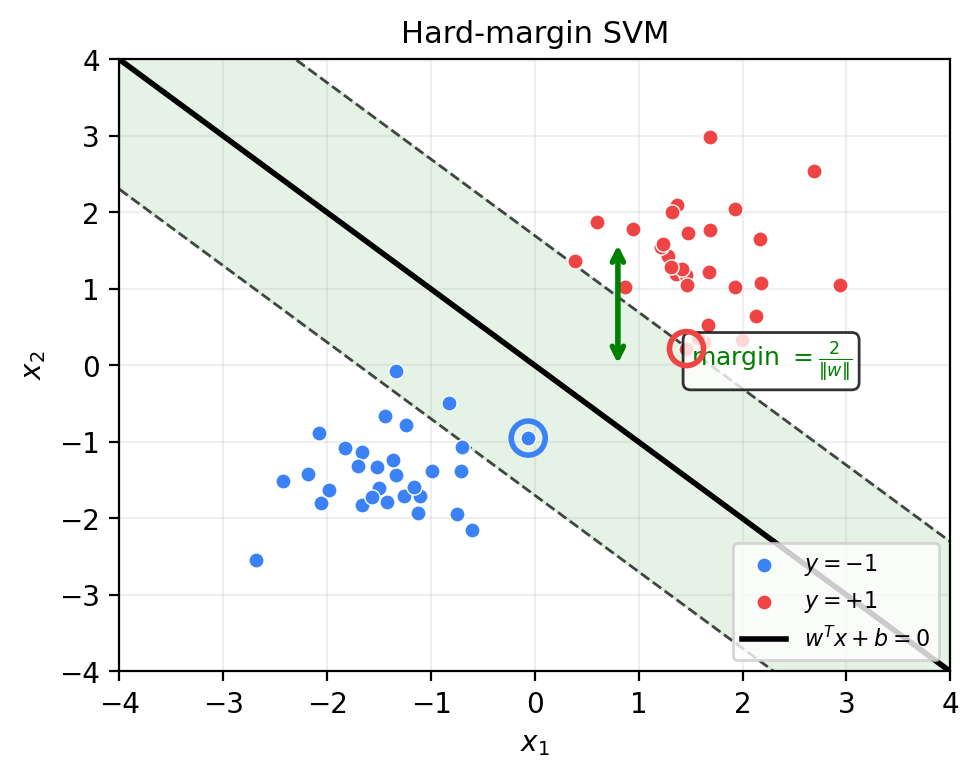
\includegraphics[width=\linewidth]{img/svm_margin}
                \vspace{0.2cm}
                Margin lớn $\Rightarrow$ VC dim nhỏ $\Rightarrow$ cận trên $R(f)$ chặt hơn.
            \end{exampleblock}

            \begin{alertblock}{Nguyên lý}
                \begin{itemize}
                    \item SVM \textbf{tối đa hoá margin} $\Leftrightarrow$ tối thiểu VC dimension.
                    \item Đây là nguyên lý \textbf{Structural Risk Minimization}.
                \end{itemize}
            \end{alertblock}
        \end{column}
    \end{columns}
\end{frame}

% ============================================================
% SLIDE 14: SVM - Trường hợp khả tách và không khả tách
% ============================================================

\begin{frame}[shrink=40]{SVM - Trường hợp khả tách và không khả tách}
    \begin{columns}[T]
        \begin{column}{0.7\textwidth}
            \begin{block}{Hard-margin vs Soft-margin SVM}
                \textbf{(a) Hard-margin} (dữ liệu khả tách tuyến tính):
                \begin{align*}
                    \min_{w,b} \quad & \frac{1}{2}\|w\|^2 \\
                    \text{s.t.} \quad & y_i(w^Tx_i + b) \geq 1, \;\; \forall i
                \end{align*}
                Margin $= \dfrac{2}{\|w\|}$. Tối thiểu $\|w\|^2$ $\equiv$ tối đa margin.

                \vspace{0.2cm}
                \textbf{(b) Soft-margin} (dữ liệu \textbf{không} khả tách):
                \begin{align*}
                    \min_{w,b,\xi} \quad & \frac{1}{2}\|w\|^2 + C\sum_{i=1}^{N}\xi_i \\
                    \text{s.t.} \quad & y_i(w^Tx_i + b) \geq 1 - \xi_i, \;\; \xi_i \geq 0
                \end{align*}

                $\xi_i$: \textbf{slack variable} -- cho phép vi phạm margin.\newline
                $C$: tham số điều chỉnh trade-off giữa margin lớn và vi phạm ít.

                \vspace{0.2cm}
                \textbf{Bài toán đối ngẫu (Dual):}
                $$ \max_{\alpha} \sum_{i}\alpha_i - \frac{1}{2}\sum_{i,j}\alpha_i\alpha_j y_i y_j x_i^Tx_j $$
                $$ \text{s.t.} \quad 0 \leq \alpha_i \leq C, \quad \sum_i \alpha_i y_i = 0 $$
            \end{block}
        \end{column}

        \begin{column}{0.28\textwidth}
            \begin{exampleblock}{Ví dụ: SVM trong trường hợp không khả tách}
                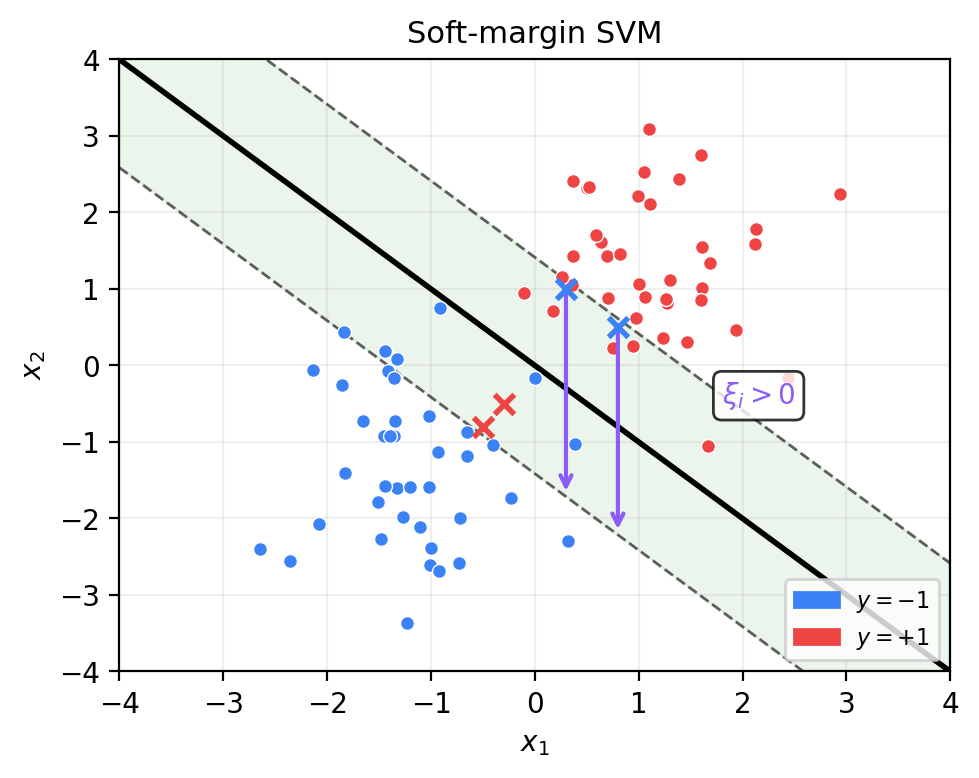
\includegraphics[width=\linewidth]{img/svm_soft_margin}
            \end{exampleblock}

            \begin{alertblock}{Nguyên lý}
                \begin{itemize}
                    \item $\alpha_i > 0$ chỉ tại \textbf{support vectors} (điểm nằm trên hoặc vi phạm margin).
                    \item $C \to \infty$: hard-margin. $C$ nhỏ: margin rộng, chấp nhận nhiều vi phạm.
                    \item Dạng đối ngẫu chỉ phụ thuộc $x_i^Tx_j$ $\Rightarrow$ mở rộng sang \textbf{Kernel trick}.
                \end{itemize}
            \end{alertblock}
        \end{column}
    \end{columns}
\end{frame}

% ============================================================
% SLIDE 15: Đánh giá kết quả phân lớp
% ============================================================

\begin{frame}[shrink=40]{Đo lường kết quả phân lớp: Confusion Matrix}
    \begin{columns}[T]
        \begin{column}{0.7\textwidth}
            \begin{block}{Confusion Matrix và các chỉ số}
                \textbf{Confusion Matrix} cho phân lớp nhị phân:

                \vspace{0.2cm}
                \begin{center}
                \begin{tabular}{c|cc}
                    & Predicted $+$ & Predicted $-$ \\
                    \hline
                    Actual $+$ & \textbf{TP} & FN \\
                    Actual $-$ & FP & \textbf{TN} \\
                \end{tabular}
                \end{center}

                \vspace{0.3cm}
                \textbf{Các chỉ số đánh giá:}
                \begin{itemize}
                    \item \textbf{Accuracy} $= \dfrac{TP + TN}{TP + TN + FP + FN}$
                    \item \textbf{Precision} $= \dfrac{TP}{TP + FP}$ ("dự đoán $+$ đúng bao nhiêu?")
                    \item \textbf{Recall (Sensitivity)} $= \dfrac{TP}{TP + FN}$ ("bắt được bao nhiêu $+$ thực?")
                    \item \textbf{F1-score} $= \dfrac{2 \cdot Precision \cdot Recall}{Precision + Recall}$
                    \item \textbf{Specificity} $= \dfrac{TN}{TN + FP}$
                \end{itemize}
            \end{block}
        \end{column}

        \begin{column}{0.28\textwidth}
            \begin{exampleblock}{Ví dụ: Confusion Matrix}
                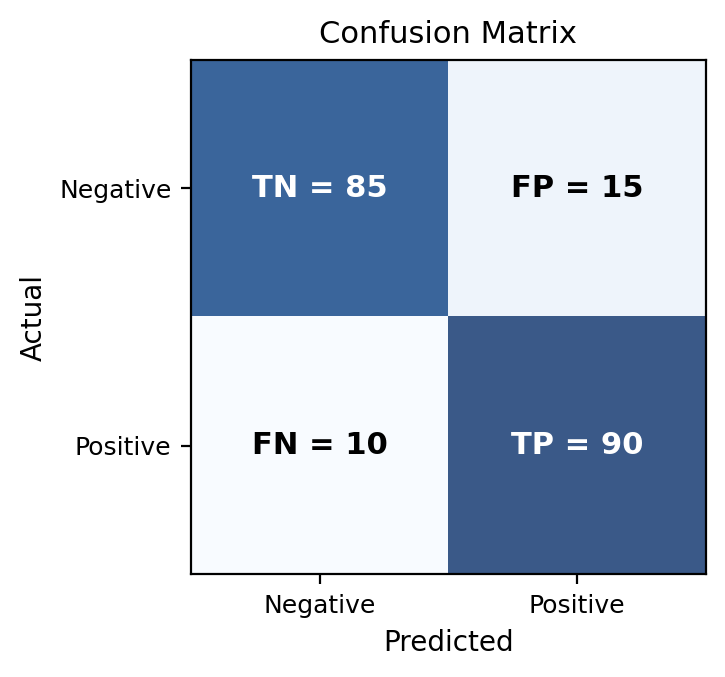
\includegraphics[width=\linewidth]{img/confusion_matrix}
            \end{exampleblock}

            \begin{alertblock}{Nguyên lý}
                \begin{itemize}
                    \item \textbf{Accuracy} không đủ khi dữ liệu \textbf{mất cân bằng}.
                    \item Precision--Recall trade-off: tăng ngưỡng $\Rightarrow$ Precision $\uparrow$, Recall $\downarrow$.
                \end{itemize}
            \end{alertblock}
        \end{column}
    \end{columns}
\end{frame}

% ============================================================
% SLIDE 16: Confidence interval cross-validation và p-value cho accuracy + p-value cho ROC - AUC
% ============================================================

\begin{frame}[shrink=40]{Đo lường kết quả phân lớp: ROC -- AUC và Cross-Validation}
    \begin{columns}[T]
        \begin{column}{0.58\textwidth}
            \begin{block}{ROC Curve và AUC}
                \textbf{ROC} (Receiver Operating Characteristic):
                \begin{itemize}
                    \item Trục $x$: \textbf{FPR} $= \frac{FP}{FP + TN}$ \quad (1 -- Specificity)
                    \item Trục $y$: \textbf{TPR} $= \frac{TP}{TP + FN}$ \quad (Recall)
                \end{itemize}

                \textbf{AUC} (Area Under ROC Curve):
                $$ AUC = \int_0^1 TPR(t)\,d(FPR(t)) \in [0, 1] $$
                $AUC = 0.5$: ngẫu nhiên. $AUC = 1$: hoàn hảo.

                \vspace{0.3cm}
                \textbf{$k$-fold Cross-Validation:}
                \begin{enumerate}
                    \item Chia dữ liệu thành $k$ phần bằng nhau.
                    \item Lần lượt dùng 1 phần làm test, $k-1$ phần làm train.
                    \item Tính trung bình các chỉ số qua $k$ lần.
                \end{enumerate}

                \textbf{Khoảng tin cậy} cho accuracy $\hat{p}$:
                $$ \hat{p} \pm z_{\alpha/2}\sqrt{\frac{\hat{p}(1-\hat{p})}{N}} $$
            \end{block}
        \end{column}

        \begin{column}{0.4\textwidth}
            \begin{exampleblock}{Ví dụ: ROC Curve}
                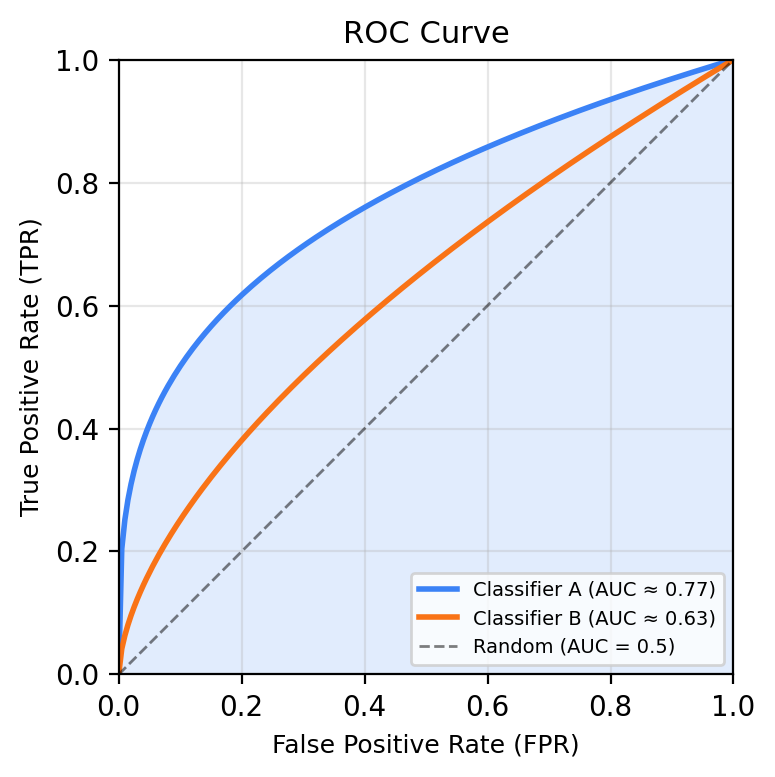
\includegraphics[width=\linewidth]{img/roc_auc}
            \end{exampleblock}

            \begin{alertblock}{Nguyên lý}
                \begin{itemize}
                    \item AUC: đánh giá \textbf{tổng thể} khả năng phân lớp, không phụ thuộc ngưỡng.
                    \item Cross-validation: ước lượng \textbf{hiệu suất tổng quát hoá} (generalisation).
                \end{itemize}
            \end{alertblock}
        \end{column}
    \end{columns}
\end{frame}